In Chapter~\ref{chap:bilinear}, we have seen the notions of bilinear complexity
and symmetric bilinear complexity. We now investigate even stronger
notions of symmetry, allowing to have very short representations of a bilinear
map.

\minitoc

% TODO
% ====
%
% Find a nice picture to put here to illustrate something in link with the
% chapter.
%
% Note
% ====
%
% It could be an illustration of the exhaustive search tree with the rank
% technique that allows to delete some branches, a nice picture of that just
% to be ble to understand how much it deletes would be very nice imho

\clearpage
\section{Symmetric and hypersymmetric fomulas}
% Table of content
% ================
%
% - Recall of the definition of symmetric
% - Existence and lemma for the symmetric case
% - non degenerate bilinear form, link with the trace, but not only
% - Link between symmetric and hypersymmetric in smaller dimension
% - Galois invariance
% - Comment for the case of the particular algebras we study, what is known and
%   what is not
%
% Comment
% =======
%
% Comment about the trisymmetric formulas, it is true that F_4/F_2 can be
% represented by a trisymmetric formula but it is not the case for F_8/F_2. We
% should check the lemma saying something on the existence of the trisymmetric
% decomposition, but it is probably just simpler.

Let $\K$ be a finite field, $V_1$, $V_2$ and $W$ three finite-dimensional $\K$-vector
space and
\[
  \Phi:V_1\times V_2\to W
\]
a bilinear map. Recall Definition~\ref{defi:bilinear-formula}:
\[
  \Phi(x, y) = \sum_{j=1}^t\varphi_j(x)\psi_j(y)w_j,
\]
where for all $1\leq j\leq t$, $\varphi_j\in V_1^\vee$ and $\phi_j\in V_2^\vee$ are linear forms and
$w_j\in W$ is a vector, is called a \emph{bilinear formula} of length $t$. If
the spaces $V_1$ and $V_2$ are equal and if the bilinear map $\Phi$ is
symmetric, \ie if for all $x, y\in V$
\[
  \Phi(x, y) = \Phi(y, x),
\]
we can investigate the existence of formulas satisfying the same condition of
symmetry, \ie formulas where for all $1\leq j\leq t$, $\varphi_j=\psi_j$,
resulting in \emph{symmetric} bilinear form:
\[
  \Phi(x, y) = \sum_{j=1}^t\varphi_j(x)\varphi_j(y)w_j.
\]
In fact, we can define other interesting types of symmetries, but it is useful
to first generalize the notions that we saw in Chapter~\ref{chap:bilinear} to
higher dimensions.
\subsection{Generalization to multilinear maps}
The definitions of bilinear formula and bilinear complexity are not bound to the
bilinear case and can be generalized to arbitrary dimension. These general
definitions will be used in Section~\ref{subsec:trisym} to define
\emph{hypersymmetric} complexity.
\begin{defi}[Multilinear formula]
Let $V_1, V_2, \dots, V_s$ and $W$ be $s+1$ finite-dimensional $\K$-vector
spaces and
\[
  \Phi:V_1\times V_2\times\dots\times V_s\to W
\]
an $s$-linear map. A \emph{multilinear formula}, or \emph{multilinear
decomposition}, or \emph{multilinear algorithm} of length $t$ for $\Phi$ is a
collection of $s\times t$ linear forms $\varphi_1^{(1)}, \varphi_2^{(1)}, \dots,
\varphi_t^{(1)}\in V_1^\vee$ up to $\varphi_1^{(s)}, \varphi_2^{(s)}, \dots,
\varphi_t^{(s)}\in V_s^{\vee}$ and $t$ vectors $w_1, \dots, w_t$, such that for all $x_1\in V_1, \dots, x_s\in
V_s$, we have
\[
  \Phi(x_1, \dots, x_s) =
  \sum_{j=1}^t\varphi_j^{(1)}(x_1)\dots\varphi_j^{(s)}(x_s)w_j.
\]
\end{defi}
\begin{defi}[Multilinear complexity]
Let $V_1, V_2, \dots, V_s$ and $W$ be $s+1$ finite-dimensional $\K$-vector
spaces and
\[
  \Phi:V_1\times V_2\times\dots\times V_s\to W
\]
an $s$-linear map. The \emph{multilinear complexity} $\mu(\Phi)$ of $\Phi$ is the
minimal length $t$ of a multilinear formula for $\Phi$.
\end{defi}
As in the case of bilinear complexity, the multilinear complexity $\mu(\Phi)$ of a
multilinear map $\Phi$ can also be defined as the rank of the tensor in 
\[
  V_1^\vee\otimes\dots\otimes V_s^\vee\otimes W
\]
corresponding to $\Phi$, see Example~\ref{ex:bilinear-complexity} for an
illustration of this correspondence in the bilinear case. In the case where
\[
  V_1 = V_2 = \dots = V_s,
\]
symmetric formulas and
symmetric complexity can also be generalized when $\Phi$ is a \emph{symmetric}
multilinear map, \ie when for all permutation $\sigma\in\mathfrak S_s$ and for
all vectors $x_1, \dots, x_s\in V$, we have
\[
  \Phi(x_1, \dots, x_s) = \Phi(\sigma(x_1), \dots, \sigma(x_s)).
\]
\begin{defi}[Symmetric multilinear formula]
Let $V$ and $W$ be two finite-dimensional $\K$-vector
spaces and
\[
  \Phi:\underset{\textrm{$s$ times}}{\underbrace{V\times\dots\times V}}\to W
\]
a symmetric $s$-linear map. A \emph{symmetric multilinear formula}, or
\emph{symmetric multilinear
decomposition}, or \emph{symmetric multilinear algorithm} of length $t$ for $\Phi$ is a
collection of $t$ linear forms $\varphi_1, \varphi_2, \dots,
\varphi_t\in V^\vee$ and $t$ vectors $w_1, \dots, w_t$, such that for all $x_1, \dots, x_s\in
V$, we have
\[
  \Phi(x_1, \dots, x_s) =
  \sum_{j=1}^t\varphi_j(x_1)\dots\varphi_j(x_s)w_j.
\]
\end{defi}
\begin{defi}[Symmetric multilinear complexity]
Let $V$ and $W$ be two finite-dimensional $\K$-vector
spaces and
\[
  \Phi:\underset{\textrm{$s$ times}}{\underbrace{V\times\dots\times V}}\to W
\]
a symmetric $s$-linear map. The \emph{symmetric multilinear complexity} $\musym(\Phi)$ of $\Phi$ is the
minimal length $t$ of a symmetric multilinear formula for $\Phi$. If no such
formula exists, we set
\[
  \musym(\Phi) = \infty.
\]
\end{defi}
Contrary to the bilinear case, some symmetric multilinear maps do not admit a symmetric
decomposition, but the problem of whether a symmetric multilinear map admits
a symmetric multilinear formula is well understood and follows from
Theorem~\ref{thm:symmetric-formula}.
\begin{thm}[{\cite[Thm.~A.7]{Randriam15}}]\label{th:criterion}
\label{thm:symmetric-formula}
Let $\Phi:V^s\to W$ be a $s$-linear map between finite dimensional vector spaces over $\mathbb{F}_q$.
Then $\Phi$ admits a symmetric decomposition if and only if $\Phi$ is \emph{Frobenius-symmetric},
\ie if and only if it is symmetric and one of the following two conditions holds:
\begin{itemize}
\item $s\leq q$
\item $s\geq q+1$ and for all $u,v,z_1,\dots,z_{s-q-1}$ in $V$,
\[
\Phi(\underset{\textrm{$q$ times}}{\underbrace{u,\dots,u}},v,z_1,\dots,z_{s-q-1})=\Phi(u,\underset{\textrm{$q$ times}}{\underbrace{v,\dots,v}},z_1,\dots,z_{s-q-1}).
\]
\end{itemize}
\end{thm}

\subsection{Trisymmetric and hypersymmetric complexity}
\label{subsec:trisym}

Under even stricter conditions, we can study the existence of even more
symmetric formulas. These formulas allow to describe a multilinear map with
fewer elements, and thus give a compact definition of the map. Since the
symmetry conditions are stronger there are fewer such formulas, and as a
consequence the search space is smaller. Thus, we expect algorithms to be
faster, as was the case when using Barbulescu \etal algorithm
(Algorithm~\ref{algo:BDEZ}) to find symmetric formulas. Let us define those
``stricter conditions''. Let
\[
  \Phi:V^s\to V
\]
be an $s$-linear symmetric map, \ie we additionnaly ask that $W=V$. We also
assume that $V$ has a non-degenerate symmetric bilinear form, that we write as a
scalar product
\[
 \begin{array}{ccc}
 V\times V &\to&\K\\
 (v,w)&\mapsto&\ps{v}{w}.
 \end{array}
\]
In that case, we know that the vector space $V$ is isomorphic to its dual space
$V^\vee$:
\[
  V\cong V^\vee,
\]
\ie for each linear form $\varphi\in V^\vee$, there exist a unique vector $a\in
V$ such that for all $x\in V$, we have
\[
  \varphi(x) = \ps{a}{x}.
\]
Under these conditions, we can now write a symmetric formula for $\Phi$ as
\[
  \Phi(x, y) = \sum_{j=1}^t\ps{a_i}{x}\ps{a_i}{y}w_j
\]
where for all $1\leq j\leq t$, $a_j\in V$ is a vector of $V$. As a consequence,
we can also describe a symmetric formula for $\Phi$ as the data of vectors
$(a_j)_{1\leq j\leq t}$ and $(w_j)_{1\leq j\leq t}$. In order to have an even
more compact description of $\Phi$, one can ask for the vectors $w_j$ to be
proportional to $a_i$, leading to the definition of hypersymmetric
formula.
% Note
% ====
%
% But is that really natural? Wouldn't it be better to say that we would like
% the a_i and the b_i to be equal? 
%
% TODO
% ====
%
% Maybe change this to include the case a_i = b_i and discuss it a little, or
% maybe not, we'll see.
%
% Remark
% ======
%
% If this is presented, it could be nice to have the tensor point of view, with
% a decomposition with the same elements three times being then very clear.

\begin{defi}[Hypersymmetric formula]
Let $V$ a finite-dimensional $\K$-vector
spaces equipped with a saclar product and
\[
  \Phi:\underset{\textrm{$s$ times}}{\underbrace{V\times\dots\times V}}\to W
\]
a symmetric $s$-linear map. A \emph{hypersymmetric formula}, or
\emph{hypersymmetric decomposition}, or \emph{hypersymmetric algorithm} of length $t$ for $\Phi$ is a
collection of $t$ vectors $a_1, \dots, a_t\in V$ and $t$ scalars $\lambda_1,
\dots, \lambda_t\in\K$, such that for all $x_1, \dots, x_s\in
V$, we have
\[
  \Phi(x_1, \dots, x_s) =
  \sum_{j=1}^t\lambda_j\ps{a_j}{x_1}\dots\ps{a_j}{x_s}a_j.
\]
\end{defi}
\begin{defi}[Hypersymmetric complexity]
Let $V$ be a finite-dimensional $\K$-vector spaces equipped with a saclar product
and
\[
  \Phi:\underset{\textrm{$s$ times}}{\underbrace{V\times\dots\times V}}\to W
\]
a symmetric $s$-linear map. The \emph{hypersymmetric complexity} $\muhyp(\Phi)$ of $\Phi$ is the
minimal length $t$ of a hypersymmetric formula for $\Phi$. If no such
formula exists, we set
\[
  \muhyp(\Phi) = \infty.
\]
\end{defi}
\begin{ex}
  \label{ex:trisymmetric-formula}
  We take the same case as in Example~\ref{ex:bilinear-complexity}, but viewed
  a bit differently. Let $\K=\mathbb{F}_2$ and 
  \[
    V=\mathbb{F}_4\cong\mathbb{F}_2[T]/(T^2+T+1)\cong\mathbb{F}_2(\zeta)
  \]
  seen as a $\mathbb{F}_2$-vector space of dimension $2$ using the base $(1,
  \zeta)$. The $\mathbb{F}_2$-bilinear map $\Phi$ that we
  consider is the product in $\mathbb{F}_4$:
  \[
 \begin{array}{cccc}
   \Phi: & \mathbb{F}_4\times \mathbb{F}_4 &\to&\mathbb{F}_4\\
 &(x,y)&\mapsto&xy.
 \end{array}
  \]
  We also consider the non-degenerate symmetric bilinear form
\[
 \begin{array}{ccc}
   \mathbb{F}_4\times \mathbb{F}_4 &\to&\mathbb{F}_2\\
 (v,w)&\mapsto&\tr(vw),
 \end{array}
\]
where $\tr$ is the trace of the field extension $\mathbb{F}_4/\mathbb{F}_2$,
and we write
\[
  \tr(xy) = \ps{x}{y}.
\]
If $x = x_0 + x_1\zeta\in\mathbb{F}_4$ is an element in the extension field, we have $\tr(x) = x_1$, and if $y = y_0
+ y_1\zeta\in\mathbb{F}_4$ is another element, then their product is
\[
  xy = x_0y_0 + x_1y_1 + (x_0y_1 + x_1y_0 + x_1y_1)\zeta.
\]
We also see that
\[
\left\{ 
  \begin{array}{lll}
    \ps{1}{x}\ps{1}{y} &=& x_1y_1 \\
    \ps{1+\zeta}{x}\ps{1+\zeta}{y} &=& x_0y_0 \\
    \ps{\zeta}{x}\ps{\zeta}{y} &=& (x_0+x_1)(y_0+y_1)
  \end{array}
\right.
\]
and thus we have
\[
  xy =
  \ps{1}{x}\ps{1}{y}\cdot1+\ps{1+\zeta}{x}\ps{1+\zeta}{y}\cdot(1+\zeta)+\ps{\zeta}{x}\ps{\zeta}{y}\cdot\zeta.
\]
This is an hypersymmetric formula of length $3$, and we can prove that there are
no formulas of length $2$, so we have
\[
  \muhyp(\Phi) = 3.
\]
This is in fact the very same formula as in
Example~\ref{ex:bilinear-complexity}.
\end{ex}
In order to investigate the existence of hypersymmetric decompositions, we
remark that there is a natural link between hypersymmetric decompositions of 
the $s$-linear map
\[
  \Phi:V^s\to V
\]
and symmetric decompositions of the $(s+1)$-linear form $\widetilde\Phi$ defined by
\[
  \begin{array}{llll}
    \widetilde\Phi:&V^{s+1}&\to&\K\\
    &(x_1, \dots, x_{s+1})&\mapsto&\ps{\Phi(x_1, \dots, x_s)}{x_{s+1}}
  \end{array}
\]
in the sense of~Lemma~\ref{lm:link-hyp-sym}. Moreover, we say that the
$s$-linear map $\Phi$ is \emph{hypersymmetric} if the associated $(s+1)$-linear
form $\widetilde\Phi$ is symmetric.
\begin{lm}
  \label{lm:link-hyp-sym}
  Let $V$ a $\K$-vector space and 
  \[
    \Phi:V^s\to V
  \]
  a symmetric $s$-linear map. 
Elements $(a_j)_{1\leq j\leq t}$ in $V$ and scalars $(\lambda_j)_{1\leq j\leq t}$ in $\K$ define a hypersymmetric formula for the $s$-linear map $\Phi$,
\[
\Phi(x_1,\dots,x_s)=\sum_{j=1}^{t}\lambda_j\ps{a_j}{x_1}\cdots\ps{a_j}{x_t}a_j,
\]
if and only if they define a symmetric formula for the $(s+1)$-linear form $\widetilde{\Phi}$,
\[
\widetilde{\Phi}(x_1,\dots,x_s,x_{s+1})=\sum_{j=1}^{t}\lambda_i\ps{a_j}{x_1}\cdots\ps{a_j}{x_t}\ps{a_j}{x_{s+1}}.
\]

Thus, $\Phi$ admits a hypersymmetric formula if and only if $\widetilde{\Phi}$ is Frobenius-symmetric (in the sense of Theorem~\ref{thm:symmetric-formula}),
and we have
\[
\muhyp(\Phi)=\musym\left(\widetilde{\Phi}\right).
\]

In particular, if $q\geq s+1$, then any hypersymmetric $s$-linear map over $\mathbb{F}_q$ admits a hypersymmetric formula.
\end{lm}
\begin{proof}
  Assume that $\Phi$ admits a hypersymmetric decomposition, such that for all
  $x_1, \dots, x_s\in V$, we have
  \[
    \Phi(x_1,\dots,x_s)=\sum_{j=1}^{t}\lambda_i\ps{a_j}{x_1}\cdots\ps{a_j}{x_t}a_j,
  \]
  then, by taking the scalar product with any $x_{s+1}$, we obtain
\[
  \ps{\Phi(x_1, \dots,
  x_s)}{x_{s+1}}=\widetilde{\Phi}(x_1,\dots,x_s,x_{s+1})=\sum_{j=1}^{t}\lambda_i\ps{a_j}{x_1}\cdots\ps{a_j}{x_t}\ps{a_j}{x_{s+1}},
\]
which defines a symmetric decomposition for $\widetilde\Phi$. In the other
direction, assume that $\widetilde\Phi$ admits a symmetric decomposition, such
that for all $x_1, \dots, x_{s+1}\in V$, we have
\[
\widetilde{\Phi}(x_1,\dots,x_s,x_{s+1})=\sum_{j=1}^{t}\lambda_i\ps{a_j}{x_1}\cdots\ps{a_j}{x_t}\ps{a_j}{x_{s+1}}.
\]
It can also be written as
\[
  \ps{\Phi(x_1, \dots,
  x_s)}{x_{s+1}}=\ps{\sum_{j=1}^t\lambda_j\ps{a_j}{x_1}\cdots\ps{a_j}{x_s}a_j}{x_{s+1}},
\]
so that we have
\[
  \ps{\Phi(x_1, \dots,
  x_s)-\sum_{j=1}^t\lambda_j\ps{a_j}{x_1}\cdots\ps{a_j}{x_s}}{x_{s+1}}=0.
\]
Since the scalar product $\ps{\cdot}{\cdot}$ is non-degenerate, it means that
  \[
    \Phi(x_1,\dots,x_s)=\sum_{j=1}^{t}\lambda_i\ps{a_j}{x_1}\cdots\ps{a_j}{x_t}a_j.
  \]
  Hence $\Phi$ admits a hypersymmetric decomposition. The other assertions
  follow.
\end{proof}
The most important case is arguably the bilinear case, where $s=2$, because it
was thoroughly studied. For that reason, we sometimes replace the word
hypersymmetric by \emph{trisymmetric} in that particular case, because of the
form of the formulas
\[
  \Phi(x, y) = \sum_{j=1}^t\lambda_j\ps{a_j}{x}\ps{a_j}{y}a_j
\]
that includes the same element $a_j$ three times, and we write $\mutri(\Phi)$
instead of $\muhyp(\Phi)$. Lemma~\ref{lm:link-hyp-sym} states that, if $q\geq3$, a
trisymmetric map $\Phi$ always admits a trisymmetric decomposition.

\subsection{Galois invariance}

An other type of interesting decompositions is Galois invariant decompositions.
It is motivated by the study of group actions on the set of decompositions, that
can sometimes be used to cut branches in the search tree of the algorithms.
% TODO
% ====
%
% Link that with BDEZ stab, the version using automorphisms, and Covanov.
Let 
\[
 \begin{array}{cccc}
   \sigma: & V\times V &\to&V\\
 &x&\mapsto&x^\sigma
 \end{array}
\]
be a $\K$-automorphism of $V$ that respects the scalar product, \ie for all $x,
y\in V$, we have
\[
  \ps{x^\sigma}{y^\sigma} = \ps{x}{y}.
\]
Then, if $\sigma$ is also compatible with some studied multilinear map $\Phi$, it induces
an action on the set of decomposition, as explained in
Lemma~\ref{lm:action-sym}.
\begin{lm}
  \label{lm:action-sym}
  Let $V$ a finite-dimensional $\K$-vector space and
  \[
    \Phi:V^s\to V
  \]
  a symmetric $s$-linear map that is compatible with $\sigma$, \ie for all $x_1,
  \dots, x_s$ in $V$, we have
  \[
    \Phi(x_1^\sigma, \dots, x_s^\sigma) = \Phi(x_1, \dots, x_s)^\sigma.
  \]
  If $(a_j)_{1\leq j \leq t}$ and $(b_j)_{1\leq j \leq t}$ define a symmetric
  formula for $\Phi$
  \[
    \Phi(x_1, \dots, x_s) = \sum_{j=1}^t\ps{a_j}{x_1}\dots\ps{a_j}{x_s}b_j,
  \]
  then $(a_j^\sigma)_{1\leq j\leq t}$ and $(b_{j}^\sigma)_{1\leq j\leq t})$ also
  define a symmetric formula for $\Phi$
  \[
    \Phi(x_1, \dots, x_s) =
    \sum_{j=1}^t\ps{a_j^\sigma}{x_1}\dots\ps{a_j^\sigma}{x_s}b_j^\sigma.
  \]
\end{lm}
\begin{proof}
 Assume that we have a symmetric decomposition for $\Phi$, with the same
 notations as in the Lemma. First, notice that for every $x,y\in V$, we have
 \[
   \ps{x^\sigma}{y} = \langle{x},{y^{\sigma^{-1}}}\rangle.
 \]
 Then, it follows that
 \begin{align*}
   \Phi(x_1, \dots, x_s) &= \Phi(x_1^{\sigma^{-1}}, \dots,
   x_{s}^{\sigma^{-1}})^\sigma\\
   &=
   (\sum_{j=1}^t\langle{a_j},{x_1^{\sigma^{-1}}}\rangle\dots\langle{a_j},{x_s^{\sigma^{-1}}}\rangle
   b_j)^\sigma\\
   &= \sum_{j=1}^t\ps{a_j^{\sigma}}{x_1}\dots\ps{a_j^\sigma}{x_s}b_j^\sigma.
 \end{align*}
 Thus we have a new symmetric formula for $\Phi$.
\end{proof}
When this action, does not change the formula, we then say that it is
$\sigma$-invariant.
\begin{defi}[$\sigma$-invariance]
  Let $(a_j)_{1\leq j\leq t}$ and
$(b_j)_{1\leq j\leq t}$ define a symmetric formula for $\Phi$
  \[
    \Phi(x_1, \dots, x_s) = \sum_{j=1}^t\ps{a_j}{x_1}\dots\ps{a_j}{x_s}b_j.
  \]
We say that this
formula is $\sigma$-invariant if it is the same as the formula defined by
$(a_j^\sigma)_{1\leq j\leq t}$ and $(b_j^\sigma)_{1\leq j\leq t}$,
\ie if there is a permutation $\pi\in\mathfrak S_t$ of $\{1,\dots,t\}$ such that
$(a_j^\sigma,b_j^\sigma)=(a_{\pi(j)},b_{\pi(j)})$ for all $j$. This also applies
to hypersymmetric formulas, setting $b_j=\lambda_j a_j$. 
\end{defi}
\begin{ex}
  In fact, the trisymmetric formula seen in
  Example~\ref{ex:trisymmetric-formula} was already $\sigma$-invariant. Recall
  that we work in $\mathbb{F}_4$, defined by
  \[
   \mathbb{F}_4\cong\mathbb{F}_2[T]/(T^2+T+1)\cong\mathbb{F}_2(\zeta),
  \]
  and we take
\[
  \tr(xy) = \ps{x}{y}.
\]
The $\mathbb{F}_2$-automorphism that we consider is the Frobenius automorphism
\[
  \begin{array}{cccc}
    \sigma: & \mathbb{F}_4 & \to & \mathbb{F}_4 \\
    & x & \mapsto & x^2.
  \end{array}
\]
We still have, for all $x, y\in\mathbb{F}_4$
\[
  xy =
  \ps{1}{x}\ps{1}{y}\cdot1+\ps{1+\zeta}{x}\ps{1+\zeta}{y}\cdot(1+\zeta)+\ps{\zeta}{x}\ps{\zeta}{y}\cdot\zeta.
\]
Since
\[
\left\{ 
  \begin{array}{l}
    1^\sigma = 1 \\
    \zeta^\sigma=\zeta+1\\
    (\zeta+1)^\sigma=\zeta
  \end{array}
\right.
\]
we see that the formula is $\sigma$-invariant.
\end{ex}

\subsection{Multiplication formulas in algebras}
\label{sec:formulas-algebras}

In the previous pages, we have defined (hyper)symmetric formulas for any
multilinear map defined over some finite-dimensional $\K$-vector space.
Nevertheless, as seen in the examples, we are often interested in special
instances of multilinear maps. In fact, the map that we have in mind is almost
always the $s$-variable product of some $\K$-algebra $\A$, with $s=2$. There are
two types of algebras we are particularly interested in:
\begin{itemize}
  \item the finite field extensions $\A=\mathbb{F}_{q^m}$, in which we take the
    trace bilinear form
    \[
      \ps{x}{y}=\tr(xy)
    \]
    for our scalar product, and the Frobenius automorphism
    \[
  \begin{array}{cccc}
    \sigma: & \mathbb{F}_{q^m} & \to & \mathbb{F}_{q^m} \\
    & x & \mapsto & x^q.
  \end{array}
\]
for our $\K$-automorphism ;
\item algebras of truncated polynomials $\A = \mathbb{F}_q[T]/(T^m)$. In this
  case, we let 
  \[
  \begin{array}{cccc}
    \tau: & \A & \to & \K \\
    & \sum_{j=0}^{m-1}x_j T^j & \mapsto & x_0
  \end{array}
\]
and
\[
  \ps{x}{y} = \tau(xy).
\]
Indeed, if $x=\sum_{j=0}^{m-1}T^j$ and $y=\sum_{j=0}^{m-1}y_jT^j$, we have
\[
  \tau(x, y) = x_0y_{m-1} + x_1y_{m-2} + \dots + x_{m-1}y_0,
\]
thus $\tau$ is a non-degenerate bilinear form.
\end{itemize}
We denote by $\mutri_q(k)$ the trisymmetric bilinear complexity of the
$2$-variable product in $\mathbb{F}_{q^k}$ and by $\hmutri_q(k)$ the
trisymmetric bilinear complexity of the $2$-variable product in
$\mathbb{F}_q[T]/(T^k)$.

\section{Algorithmic search in small dimension}

In very small dimension, \eg in Examples~\ref{ex:bilinear-complexity}
and~\ref{ex:trisymmetric-formula} where we are working with $\K$-vector spaces
of dimension $2$, the search of formulas can be done by hand relatively easily
because the length of the formulas is short. Though, even in small dimension, if
the cardinality of $\K$ is large, the number of different formulas can be
big, thus making it hard to list \emph{all} different solutions. For these
reasons, it is highly desirable to \emph{algorithmically} find the formulas.
Let $V$ be a finite dimensional $\K$-vector space and $\Phi:V\times V\to V$ a bilinear map.
When wanting to list all the symmetric formulas of the form
\[
  \Phi(x, y) = \sum_{j=0}^t\varphi_j(x)\varphi_j(y)a_j,
\]
Barbulescu~\etal\!\!\!'s and Covanov's algorithms exhaustively search through
all linear forms $\varphi$, cleverly eliminating useless branches in the search
tree. Nevertheless, their methods exploit the fact that it is possible to freely
choose the vectors $a_j\in V$, independently of the linear forms $\varphi_j\in
V^\vee$. This is
no longer possible when searching for trisymmetric decompositions
\[
  \Phi(x, y) = \sum_{j=0}^t\lambda_j\ps{a_j}{x}\ps{a_j}{y}a_j,
\]
because each
linear form $\varphi\in V^\vee$ is linked with a unique vector $a\in V$ such
that for all $x\in V$
\[
  \varphi(x) = \ps{a}{x},
\]
and the choice of a linear form $\varphi_j$ with $\varphi_j(x)=\ps{a_j}{x}$
imposes the choice of the vector $a_j\in V$. We thus propose an \emph{ad hoc}
algorithm to find trisymmetric formulas, exploiting the vector space structure.

\subsection{General algorithm description}
\label{sec:general-algorithm}

In all the section, we assume that $\K=\mathbb{F}_q$ is the finite field with
$q$ elements, $V$ is a finite-dimensional $\K$-vector space equipped with a
non-degenerate bilinear form, written as a sclar product $\ps{\cdot}{\cdot}$,
and $\Phi:V\times V\to V$ is a hypersymmetric bilinear map for which we want to
compute trisymmetric decompositions
\[
  \Phi(x, y) = \sum_{j=1}^t\lambda_j\ps{a_j}{x}\ps{a_j}{y}a_j.
\]
Assume that
\[
  V\cong\K^m
\]
is a $\K$-vector space of dimension $m$, for which a basis has been chosen and
allows us to identify $V$ to $\K^m$, and
let $(b_j)_{1\leq j\leq m}$ be the bilinear forms on each coordinates, \ie for
all $x,y\in V$, we have
\[
  \Phi(x, y) = (b_1(x, y), \dots, b_m(x, y)).
\]
We have already seen that the difficulty in the trisymmetric case resides in the
fact that each linear form, or equivalently each symmetric rank $1$ bilinear
form, comes with a given vector in $V$ that dictates its impact on the different
coordinates in a trisymmetric formula. Therefore, a central idea is to
exhaustively search through vectors in $V$ instead of linear forms in $V^\vee$.
This is equivalent since 
\[
  V\cong V^\vee
\]
in this case anyway. Moreover, we search through special sets of vectors that
have easy-to-manage coordinates, \eg well-placed zeros and ones, in order to
control the impact on certain coordinates. Assume $(a_j)_{1\leq j \leq t}$ in $V$ and
$(\lambda_j)_{1\leq j \leq t}$ in $\K$ define a trisymmetric decomposition
\[
  \Phi(x, y) = \sum_{j=1}^t\lambda_j\ps{a_j}{x}\ps{a_j}{y}a_j.
\]
Without loss of generality, we can consider that every element $a_j$ is
``normalized'', \ie its first nonzero coordinate is $1$. Indeed, if we have one
\[
  a_{j_0} = 0
\]
for some $1\leq j_0 \leq t$, then we just remove one term from the formula and
we still have a trisymmetric decomposition, of length $t-1$. Now if for every
$1\leq j\leq t$, 
\[
  a_j\neq0,
\]
we let $x_j$ be the first nonzero coordinate of $a_j$ and we write
\[
  a_j = x_j \widetilde a_j.
\]
We can now write the trisymmetric formula as
\begin{align*}
  \Phi(x, y) &= \sum_{j=1}^t\lambda_j\ps{a_j}{x}\ps{a_j}{y}a_j \\
  &= \sum_{j=1}^t\lambda_j\ps{x_j\widetilde a_j}{x}\ps{x_j\widetilde
  a_j}{y}x_j\widetilde a_j \\
  &= \sum_{j=1}^t\lambda_jx_j^3\ps{\widetilde a_j}{x}\ps{\widetilde
  a_j}{y}\widetilde a_j \\
  &= \sum_{j=1}^t\widetilde \lambda_j\ps{\widetilde a_j}{x}\ps{\widetilde
  a_j}{y}\widetilde a_j,
\end{align*}
where $\widetilde\lambda_j = \lambda_jx_j^3$.
Therefore any trisymmetric formula is equivalent to a trisymmetric formula with
normalized vectors, and thus we only search for formulas with normalized
elements. In other words, for all $1\leq j\leq m$, we let
\[
  \E_j=\left\{ x=(x_1, \dots, x_k)\in V
  \,|\, \forall i\leq j-1,\,x_i=0\text{ and }x_j=1 \right\}
\]
and
\[
  \E = \bigcup_{j=1}^m\E_j,
\]
and we search for elements $a_j$ in $\E$ instead of the entire vector space $V$.
Limiting the search to $\E$ helps us in two different ways. First, it reduces
the complexity of the exhaustive search since the cardinality of $\E$ is smaller
than the cardinality of $V$. Indeed, the sets $\E_j$ are disjoint, so
\begin{align*}
  \Card\E &= \sum_{j=1}^m\Card\E_j\\
  &= \sum_{j=1}^m q^{m-j}\\
  &= \cfrac{q^m-1}{q-1},
\end{align*}
whereas
\[
  \Card V = q^m.
\]
Second, it allows a better understanding of what happens in the algorithm,
because if we have some vector
\[
  a\in\E_j
\]
for a given $1\leq j\leq m$, we know that the associated bilinear form
\[
  (x, y)\mapsto\ps{a}{x}\ps{a}{y}
\]
can only impact the coordinates $i\geq j$. Thus, we further
use the vector space structure of $V$ by searching for solutions
on each coordinate, starting with the first coordinates and vectors in $\E_1$,
then the second coordinate and vectors in $\E_2$, and so on until the last
coordinate. Let us focus on the first coordinate first and give some details.

Recall that the goal is to obtain a trisymmetric decomposition for the
hypersymmetric bilinear map $\Phi:V\times V\to V$, that is written
\[
  \Phi(x, y) = (b_1(x, y), \dots, b_m(x, y)).
\]
in the basis of $V$. We first see how to decompose the bilinear \emph{form}
$b_1$ as a sum of rank $1$ bilinear forms. Let $\B$ be the set of bilinear forms
of $V\times V$, recall that $\B$ is a $\K$-vector space of dimension $m^2$, and
that we identify $b_1$ with the $m\times m$ matrix $B_1\in\K^{m\times m}$ 
such that for all vectors $x, y\in V$, we have
\[
  b_1(x, y) = X B_1 Y^t,
\]
where $X, Y\in\K^{1\times m}$ are the row vectors representing $x$ and $y$ and
where $Y^t$ is the transposed of $y$. Let $r_1$ be the rank of $b_1$, we know
that $b_1$ can be decomposed as a sum of $r_1$ bilinear forms of rank $1$. Let
$f$ be the application mapping an element in $V$ to its associated bilinear
form:
\[
  \begin{array}{cccc}
    f: & V & \to & \B\\
    & a & \mapsto & (x, y)\mapsto\ps{a}{x}\ps{a}{y}.
  \end{array}
\]
In order to find these decompositions, we begin by exhaustively searching through scalars $\lambda_1\in\K$ and vectors
$a_1\in \E_1$ such that
\[
  r_1-1=\rank(b_1-\lambda_1 f(a_1)) < \rank(b_1)=r_1.
\]
Then, for each such couple $(\lambda_1, a_1)$, we exhaustively search through
scalars $\lambda_2\in\K$ and vectors $a_2\in \E_1$ such that
\[
  r_1-2=\rank(b_1-\lambda_1 f(a_1)-\lambda_2f(a_2)) < \rank(b_1-\lambda_1
  f(a_1))=r_1-1.
\]
We continue this process until we have $r_1$ couples $(\lambda_1, a_1), \dots,
(\lambda_{r_1}, a_{r_1})$ such that
\[
  0 = \rank(b_1-\sum_{j=1}^{r_1}\lambda_jf(a_j)) <
  \rank(\sum_{j=1}^{r_1-1}\lambda_jf(a_j)) = 1,
\]
that exactly means that
\[
  b_1 = \sum_{j=1}^{r_1}\lambda_jf(a_j),
\]
and we have found our decomposition.
In fact, we can search in a more clever way. Since the rank of $b_1$ is $r_1$
and we are looking for decompositions as a sum of exactly $r_1$ bilinear forms of
rank $1$, we must choose
couples $(\lambda_j, a_j)$ that decrease the rank of our bilinear form at each
step, otherwise we will need strictly more than $r_1$ bilinear forms of rank
$1$. Therefore, at each step, we can search only through the vectors that can
decrease the rank of the last considered bilinear form. After each choice of
$(\lambda_1, a_1)$, we will thus exhaustively search through scalars
$\lambda_2\in\K$ and vectors $a_2$ in
\[
  \E_1^{\left\{ (\lambda_1, a_1) \right\}} = \left\{
  a\in\E_1\;|\;\exists\lambda\in\K,\,\rank(b_1-\lambda f(a)) <\rank(b_1)
\right\}.
\]
Then, after each choice of $(\lambda_2, a_2)$, we will search through scalars
$\lambda_3\in\K$ and vectors $a_3$ in
\[
  \E_1^{\left\{ (\lambda_1, a_1), (\lambda_2, a_2) \right\}} = \left\{
    a\in\E_1^{ \left\{ (\lambda_1, a_1)
    \right\}}\;|\;\exists\lambda\in\K,\,\rank(b_1-\lambda_1f(a_1)-\lambda f(a))
    <\rank(b_1-\lambda_1f(a_1))
\right\},
\]
and we use the same idea until the end of the process. This strategy, used in
Algorithm~\ref{algo:mindecomp}, permits to
save a lot of time in the search because we look only at the vectors that have
the potential to decrease the rank, instead of all the vectors in $\E_1$.
\begin{algorithm}
  \caption{(Minimal decomposition)}
  \label{algo:mindecomp}
  \begin{algorithmic}[1]
    \Require{$b\in \B$ a bilinear form of rank $r$, $E\subset\E$
    the space of vectors in which to search}
    \Ensure{A list of decompositions of $b$ as a sum of bilinear forms of rank
    $1$, each decomposition represented by a set of $r$ couples $\left\{
      (\lambda_1, a_1), \dots, (\lambda_{r}, a_{r})\right\}$.}

    \Procedure{MinimalDecomposition}{$b, E, R_{\text{glob}},
    R_{\text{loc}}=\emptyset$}
    \If{$\varphi=0$}\Comment{$\rank(\varphi)=0$}
    \State $R_\text{glob}\gets R_\text{glob}\bigcup\left\{R_\text{loc}\right\}$
    \Else
    \State $\mathcal C\gets\emptyset$\Comment{$\mathcal C$ is the set of couples
    that decrease the rank}
    \ForAll{$a\in E$}
    \ForAll{$\lambda\in\K$}
  \If{$\rank(b-\lambda f(a))<\rank(b)$}
    \State $\mathcal C\gets\mathcal C\bigcup\left\{ (\lambda, a) \right\}$
    \State \textbf{break}\Comment{breaks only the inner loop}
    \EndIf
    \EndFor
    \EndFor
    \For{$i=1$ to $\Card\mathcal C$}\Comment{we note $\mathcal
      C=\left\{ (\gamma_1, c_1), \dots, (\gamma_u, c_u) \right\}$}
      \State $E'\gets\left\{ c_{i+1}, \dots, c_u \right\}$
    \State \Call{MinimalDecomposition}{$b-\gamma_i f(c_i), E', R_\text{glob},
    R_\text{loc}\cup\left\{ (\gamma_i, c_i) \right\}$}
    \EndFor
    \EndIf
    \EndProcedure

   \State $\mathcal R\gets\emptyset$
    \State \Call{MinimalDecomposition}{$b, E, \mathcal R$}
    \State \Return $\mathcal R$
  \end{algorithmic}
\end{algorithm}


For each decomposition of $b_1$
\[
  b_1(x, y) = \sum_{j=1}^{r_1}\lambda_j\ps{a_j}{x}\ps{a_j}{y}
\]
that we compute this way, we obtain
\[
  \Phi(x, y) - \sum_{j=1}^{r_1}\lambda_j\ps{a_j}{x}\ps{a_j}{y}a_j = (0, b_2'(x,
  y), \dots, b_m'(x, y)),
\]
where $b_2', \dots, b_m'\in\B$ are new bilinear forms, depending on the coordinates
of $a_1, \dots, a_{r_1}$, and where the first coordinate is $0$ because the
first coordinate of the vectors $a_1, \dots, a_{r_1}$ is always $1$. Then, we
use Algorithm~\ref{algo:mindecomp} with the bilinear form $b_2'$ of rank $r_2$ and the initial
set of vectors $\E_2$. For each decomposition of $b_2'$
\[
  b_2'(x, y) = \sum_{j=r_{1}+1}^{r_1+r_2}\lambda_j\ps{a_j}{x}\ps{a_j}{y}
\]
obtained, we have
\[
  \Phi(x, y) - \sum_{j=1}^{r_1+r_2}\lambda_j\ps{a_j}{x}\ps{a_j}{y}a_j = (0, 0,
  b_3''(x, y), \dots, b_m''(x, y)),
\]
where $b_3'', \dots, b_m''\in\B$ are again new bilinear forms, depending on the
coordinates of the elements $a_{r_1+1}, \dots, a_{r_1+r_2}$. We continue this
process on all the coordinates, such that in the end we obtain trisymmetric
decompositions of the form
\[
  \Phi(x, y) = \sum_{j=1}^t\lambda_j\ps{a_j}{x}\ps{a_j}{y}a_j.
\]
The overall strategy is described in Algorithm~\ref{algo:trisymmin}.
\begin{algorithm}
  \caption{(Trisymmetric search with minimal
  decompositions)}\label{algo:trisymmin}
  \begin{algorithmic}[1]
    \Require{$\Phi=(b_1, \dots, b_n)$ a bilinear map;
      $t\in\mathbb{N}$ an integer}
    \Ensure{A list of tri-symmetric decompositions of $\Phi$ of length up to $t$.}

    \Procedure{TriSymSearchMin}{$\Phi, t, S_\text{glob}, j=1,
    S_\text{loc}=\emptyset$}
      \If{$\Phi = 0$}
      \State $S_\text{glob}\gets S_\text{glob}\bigcup \left\{S_\text{loc}\right\}$.
      \ElsIf{$\rank(b_j)\leq t$}
        \State $\mathcal R\gets\emptyset$
        \State \Call{MinimalDecomposition}{$b_j, \E_j,
        \mathcal R$}\Comment{We have $\Phi=(b_1, \dots, b_n)$}
        \ForAll{$S\in\mathcal R$}
        \State $\Phi'\gets\Phi-\sum_{(\lambda, \alpha)\in
        S}\lambda\f(\alpha)\alpha$
        \State \Call{TriSymSearchMin}{$\Phi', t-\Card S, S_\text{glob}, j+1,
          S_\text{loc}\cup S$}
        \EndFor
      \EndIf
    \EndProcedure
    \State $\mathcal S\gets\emptyset$
    \State \Call{TriSymSearchMin}{$\Phi, t, \mathcal S$}
    \State \Return $\mathcal S$
  \end{algorithmic}
\end{algorithm}

Let $(\lambda_j)_{1\leq j\leq t}$ be some scalars in $\K$ and $(a_j)_{1\leq
j\leq t}$ some vectors in
\[
  \E=\bigcup_{j=1}^m\E_j
\]
that define an optimal trisymmetric decomposition for $\Phi$
(\ie the length of the decomposition is minimal): 
\[
  \Phi(x, y) = \sum_{j=1}^t\lambda_j\ps{a_j}{x}\ps{a_j}{y}a_j.
\]
Although the formula is optimal, it is entirely possible for the individual
coordinate decompositions to be sub-optimal. Assume that for all vectors $x,
y\in V$, we have
\[
  \Phi(x, y) = (b_1(x, y), \dots, b_m(x, y)),
\]
with $r_1$ the rank of the bilinear form $b_1\in\B$. If we have strictly more
than $r_1$ different vectors in $(a_j)_{1\leq j\leq t}$ that belong to $\E_1$,
then Algorithm~\ref{algo:trisymmin} will not find this decomposition. Indeed,
Algorithm~\ref{algo:mindecomp} only finds \emph{minimal} decompositions of $b_1$
into $r_1$ bilinear forms of rank $1$, \ie finds decompositions with exaclty
$r_1$ vectors in $(a_j)_{1\leq j\leq t}$ that are in $\E_1$. More generally, in
Algorithm~\ref{algo:mindecomp}, when working with a bilinear form $b$ of rank
$r$, it is possible that the best \emph{local} decompositions (\ie on only one
coordinate) of length $r$ are not the best in order to find \emph{global}
decompositions (\ie on all the coordinates), because of the impact the
decompositions of $b$ have on the other coordinates. For that reason, it is
important to add the option in Algorithm~\ref{algo:mindecomp} to search for
non-optimal decompositions. That is exactly what is done in
Algorithm~\ref{algo:decompmargin}: if we want to find all decompositions of some
bilinear form $b$ of rank $r$ of length $r+\mu$, with $\mu>0$, we still
exhaustively search through scalars $\lambda\in\K$ and vectors $a\in\E$, but we
allow the rank \emph{not to} decrease on $\mu$ different times. Once this number
of ``exceptions'' have all been used, we go back to the strategy previously
presented (\ie Algorithm~\ref{algo:mindecomp}).
\begin{algorithm}
  \caption{(Decomposition with margin)}\label{algo:decompmargin}
  \begin{algorithmic}[1]
    \Require{$b\in \B$ a bilinear form of rank $r$, $E\subset\E$
    the space of vectors in which to search, $\mu$ the margin, $t$ the maximum
  length of a decompositon of $b$}
    \Ensure{A list of decompositions of $b$ as a sum of at bilinear forms of rank
    $1$, each decomposition represented by a set of at most $t$ couples $\left\{
      (\lambda_1, a_1), \dots, (\lambda_{r}, a_{t})\right\}$.}

    \Procedure{DecompositionWithMargin}{$b, E, r, m, R_{\text{glob}},
    R_{\text{loc}}=\emptyset$}
    \If{$\rank b\leq t$}
    \If{$b=0$}\Comment{$\rank b=0$}
    \State $R_\text{glob}\gets R_\text{glob}\bigcup\left\{R_\text{loc}\right\}$
    \ElsIf{$m=0$}\Comment{No margin left!}
    \State \Call{MinimalDecomposition}{$\varphi, E, R_\text{glob},
    R_\text{loc}$}\Comment{"naive" strategy: Alg.~\ref{algo:mindecomp}}
   \Else
   \For{$i=1$ to $\Card E$}\Comment{We note $E=\left\{ c_1, \dots, c_u \right\}$}
   \State $E'\gets\left\{ c_{i+1}, \dots, c_u \right\}$
    \ForAll{$\lambda\in\mathbb{F}_p$}
    \State $b'\gets b-\lambda f(c_i)$
    \State $R_\text{loc}'\gets R_\text{loc}\bigcup\left\{ (\lambda, c_i)
    \right\}$
    \If{$\rank(b')<\rank(b)$}
    \State \Call{DecompositionWithMargin}{$b', E', t-1, \mu,
      R_\text{glob}, R_\text{loc}'$}
    \Else
    \State \Call{DecompositionWithMargin}{$b', E', t-1, \mu-1,
      R_\text{glob}, R_\text{loc}'$}
    \EndIf
    \EndFor
    \EndFor
    \EndIf
    \EndIf
    \EndProcedure

    \State $\mathcal R\gets\emptyset$
    \State \Call{DecompositionWithMargin}{$b, E, \mu, \mathcal S$}
    \State \Return $\mathcal R$
  \end{algorithmic}
\end{algorithm}
We let $\mu_j$ be the number of times we allow the rank not to decrease when
dealing with the $j$-th coordinate during the trisymmetric search, and we let
\[
  \mathfrak M=(\mu_1, \dots, \mu_m).
\]
We call this $m$-uple the \emph{margin} of the exhaustive search.
Algorithm~\ref{algo:trisymmargin} is then a generalization of
Algorithm~\ref{algo:trisymmin} that includes the notion of margin. In the other
direction, Algorithm~\ref{algo:trisymmin} is the special case of
Algorithm~\ref{algo:trisymmargin} with the margin
\[
  \mathfrak M = (0, \dots, 0).
\]
\begin{algorithm}
  \caption{(Trisymmetric search with margins)}
  \label{algo:trisymmargin}
  \begin{algorithmic}[1]
    \Require{$\Phi=(b_1, \dots, b_n)$ a bilinear map;
      $t\in\mathbb{N}$ an integer, $\mathfrak M$ a margin}
    \Ensure{A list of tri-symmetric decompositions of $\Phi$ with up to $t$ elements.}

    \Procedure{TriSymSearchMargin}{$\Phi, t, \mathfrak M, S_\text{glob}, j=1,
    S_\text{loc}=\emptyset$}
      \If{$\Phi = 0$}
      \State $S_\text{glob}\gets S_\text{glob}\bigcup \left\{S_\text{loc}\right\}$.
      \ElsIf{$\rank(b_j)\leq t$}
      \State $\mathcal R\gets\emptyset$\Comment{We note $\mathfrak M = (\mu_1,
      \dots, \mu_m)$}
        \State \Call{DecompositionWithMargin}{$b_j, \E_j, t, \mu_j,
        \mathcal R$}\Comment{We note $\Phi=(b_1, \dots, b_n)$}
        \ForAll{$S\in\mathcal R$}
        \State $\Phi'\gets\Phi-\sum_{(\lambda, \alpha)\in
        S}\lambda\f(\alpha)\alpha$
        \State \Call{TriSymSearchMargin}{$\Phi', t-\Card S, \mathfrak M, S_\text{glob}, j+1,
          S_\text{loc}\cup S$}
        \EndFor
      \EndIf
    \EndProcedure
    \State $\mathcal S\gets\emptyset$
    \State \Call{TriSymSearchMargin}{$\Phi, t, \mathfrak M, \mathcal S$}
    \State \Return $\mathcal S$
  \end{algorithmic}
\end{algorithm}
Algorithm~\ref{algo:trisymmargin} behaves differently, both in 
performance and in number of decompositions found, when used with a variety
of margins. Example~\ref{ex:F27} shows a simple case of this phenomenon on a
small field extension.

% TODO
% ====
%
% An example of the coordinate search algorithm that is illuminating: probably
% the example of F_{3^3} because it shows the effect of the margins and the
% number of decompositions is only 4. Also a tree showing that the rank
% decreasing technique allows to eliminate some elements in the search would be
% very nice. Maybe there is someting interesting with F_{5^2}, F_{7^2} also?
% F_{11^2} is already less interesting than F_{3^3} I think.
\begin{ex}
  \label{ex:F27}
  In order to illustrate the impact of the choice of a given margin, let us see
  the case of the extension
 \[
   \mathbb{F}_{3^3}\cong \mathbb{F}_{3}[x]/(x^3-x+1)\cong \mathbb{F}_3[z]
 \]
 over $\mathbb{F}_3$. There are $4$ tri-symmetric decomposition of length $6$ of
 the product in $\mathbb{F}_{3^4}$:
 \begin{align*}
   d_1 &=\left\{(1, z^2 + z),
  (2, z^2 + z + 1),
  (1, z^2 - z + 1),
  (1, -z^2 + 1),
  (2, -z^2 + z + 1),
  (1, -z^2 -z + 1)\right\}\\
  d_2 &= \left\{(2, z^2),
  (2, z^2 + 1),
  (1, z^2 + z + 1),
  (2, -z^2 + 1),
  (1, -z^2 + z),
  (2, -z^2 - z + 1)\right\}\\
  d_3 &= \left\{(1, z),
  (1, z + 1),
  (2, -z + 1),
  (2, z^2 + z),
  (1, -z^2 + 1),
  (1, -z^2 + z)\right\}\\
  d_4 &= \left\{ (1, z^2),
  (1, z^2 + 1),
  (2, z^2 + z),
  (2, z^2 - z + 1),
  (2, -z^2 + z),
  (1, -z^2 + z + 1).\right\}
 \end{align*}
How the elements of each decomposition fall into the sets $\E_1$, $\E_2$ or
$\E_3$ is described in Table~\ref{tab:setsEj}.
Table~\ref{tab:illustration-margins} describes which
choice of margin allows to find which decomposition. There
is a checkmark \checkmark when the algorithm succeeds in finding the
decomposition.
 \begin{table}
   \centering
\begin{tabular}{|c||ccc|}
   \hline
   \diagbox{Decomposition}{Set} & $\mathcal E_1$ & $\mathcal E_2$
   & $\mathcal E_3$ \\
   \hline
   \hline
   $d_1$ & 5 & 1 & 0 \\
   $d_2$ & 4 & 1 & 1 \\
   $d_3$ & 3 & 3 & 0 \\
   $d_4$ & 3 & 2 & 1 \\
  \hline
 \end{tabular}
 \caption{The decompositions and how many of their vectors are in each set
 $\E_1$, $\E_2$ and $\E_3$.}
\label{tab:setsEj}
 \end{table}

 \begin{table}
   \centering
 \begin{tabular}{|c||ccccc|}
   \hline
   \diagbox{\small{Decomposition}}{\small{Margin}} & $(0, 0, 0)$ & $(1, 0, 0)$
   & $(0, 1, 0)$ & $(1, 1, 0)$ & $(2, 1, 0)$ \\
   \hline
   \hline
   $d_1$ & & & & & \checkmark \\
   $d_2$ & & \checkmark & & \checkmark & \checkmark \\
   $d_3$ & & & \checkmark & \checkmark & \checkmark \\
   $d_4$ & \checkmark & \checkmark & \checkmark & \checkmark & \checkmark \\
  \hline
 \end{tabular}

   \caption{The margins and the decompositions they permit to find.}
   \label{tab:illustration-margins}
 \end{table}
\end{ex}

% TODO
% ====
%
% Some experiments with *universal* formulae? Should we talk about that in this
% section or the next?
\subsection{Implementation}

The ideas discussed in Section~\ref{sec:general-algorithm}, in particular
Algorithms~\ref{algo:decompmargin}~and~\ref{algo:trisymmargin}, were implemented
using Nemo~\cite{Nemo}, a number theory library written in the Julia programming
language~\cite{Julia}. Nemo functionnalities includes a wrapper for
Flint~\cite{Flint}, a number theory library written in the C programming
language. The code is available online at
\url{https://github.com/erou/TriSym.jl}.

\paragraph{Julia and Nemo.} Julia is a free and open-source, high-level programming language
developed since 2012, with dynamic type system and high-performance. It is
a compiled language, with a just-in-time (jit) compilation, meaning that the
compilation is almost invisible for the user but performances are comparable
with other compiled languages. It is easy to learn and to read, especially
for someone who already worked with a high-level language like Python.
There are of course many other things to say about this new language, the
interested reader can find additional informations on Julia’s
website\footnote{\url{https://julialang.org/}} and, of
course, in the documentation of the language. Julia is designed for numerical
computing, but there are many other kind of possibilities, \eg some symbolic computer algebra packages, such as
Nemo. Nemo is a computer algebra package for Julia. It aims to cover
commutative algebra, number theory and group theory. It contains wrappers
for MPIR, Flint, Arb and Antic, and other features written directly in Julia. Among
these libraries, the C library Flint (Fast library for number theory) is the
only one that we use.
One of the advantages of Julia is that it is fairly easy
to directly call C functions contained in other libraries. Therefore, all the
Nemo functions that we use in TriSym.jl are in fact Flint functions. This
provides efficiency, the main reason why we use the duo Julia/Nemo, as well
as simplicity, because we are not directly using the C programming language.
On top of that, if a Flint function is not available in Nemo, we can directly
call it from Julia. Moreover, it is also possible to write crucial parts of the code
directly in C and call the code if necessary.

\paragraph{Trisymmetric search in finite fields.}

An algorithm in our Julia library \texttt{Trisym.jl} is specially designed to
handle trisymmetric decompositions of the product in finite fields. We use a lot
of native Nemo types, that are wrappers for Flint types. Finite fields elements
are represented by univariate polynomials modulo an irreducible polynomial and
only prime field extensions
\[
  \mathbb{F}_{p^k}/\mathbb{F}_p,
\]
where $p$ is a prime number, can be considered.
There are two types used to work with finite fields in Flint: \texttt{fq} and
\texttt{fq\_nmod}, the latter only works for word-size primes $p$. Because the
algorithms for trisymmetric searchs have an exponential complexity, we focused
our implementation on finite fields with a word-size characteristic, but there
are no theoretical nor implementation obstacles preventing an
implementation with the type \texttt{fq} and arbitrary large characteristic.
Nonetheless, implementing the algorithms for any kind of extension
\[
  \mathbb{F}_{q^k}/\mathbb{F}_q,
\]
where $q$ is a prime power, would require additionnal work.
The
bilinear forms in $\mathbb{F}_{p^k}$ are represented by $k\times k$ matrices
over $\mathbb{F}_p$, and the product in $\mathbb{F}_{p^k}$ is represented by a
$k$-uple of $k\times k$ matrices. The matrix manipulations are all done by Flint using
efficient C code: it is in particular true the rank computation, that plays a central role
in Algorithm~\ref{algo:decompmargin}. We always precompute a dictionnary maping
elements in the finite field
\[
  a\in\mathbb{F}_{p^k}
\]
to the matrix representing the bilinear form
\[
  (x, y)\mapsto\ps{a}{x}\ps{a}{y}.
\]
This bilinear form is not hard to compute: it suffices to compute a
matrix-vector multiplication, but since we have to compute the same bilinear
forms several times, we prefer to store them in a dictionnary.

% TODO
% ====
%
% Discussion and measures about the speed of the algorithm(s)

\section{Asymptotic complexities}
\label{sec:asymptotic}

Parallel to the question of finding the hypersymmetric complexity of bilinear
maps over $\K$-vector spaces of small dimension, it is also of theoretical
importance to understand how these quantities asymptotically grow. In the
bilinear case, we have rather precise bounds on
\[
  \limsup_{k\to\infty}(\frac{1}{k}\mu_q(k)).
\]
In particular, these bounds imply that the bilinear complexity $\mu_q(k)$ grows
linearly in $k$. Since we have similar results for the symmetric bilinear
complexity, we also know that $\musym_q(k)$ grows linearly in $k$. A natural
question that follows is then if we can also prove that the trisymmetric
complexity
\[
  \mutri_q(k)
\]
still grows linearly in $k$. In this section, we work with either the algebra 
\[
  \A=\mathbb{F}_{q^k}\text{ or }\A=\mathbb{F}_q[T]/(T^k),
\]
seen as an algebra over $\K=\mathbb{F}_q$, and
equipped with the scalar product 
\[
  \ps{x}{y} = \tau(xy)
\]
introduced in
Section~\ref{sec:formulas-algebras}, \ie
\begin{itemize}
  \item if $\A=\mathbb{F}_{q^k}$, $\tau=\tr$ is the trace map;
  \item if $\A = \mathbb{F}_{q}[T]/(T^k)$ and $x=\sum_{j=0}^{k-1}x_jT^j$, then
    $\tau(x) = x_0$ is the map sending an element to its constant coefficient.
\end{itemize}
Our aim is to show that the trisymmetric bilinear complexities $\mutri_q(k)$ and $\hmutri_q(k)$ grow linearly as $k\to\infty$.
Our proof will involve higher multilinear maps, and in turn, give results for them as well.

For any $t$ we define the $t$-multilinear multiplication map in $\A$ over $\K$
\[
\begin{array}{cccc}
m_t:&\A^t&\to&\A\\
&(x_1,\dots,x_t)&\mapsto&x_1\cdots x_t
\end{array}
\]
and the $t$-multilinear trace form
\[
\begin{array}{cccc}
\tau_t=\tau\circ m_t:&\A^t&\to&\A\\
&(x_1,\dots,x_t)&\mapsto&\tau(x_1\cdots x_t).
\end{array}
\]
If needed, we will write ${m_t}^{\A/\K}$ or ${\tau_t}^{\A/\K}$ to keep $\A$ and $\K$ explicit. 
The (symmetric) multilinear complexity of $m_t$ has been considered in \cite{Bshouty13} in relation with the theory of testers.

\begin{lm}
\label{lm:hyp<sym+1}
The map $m_t$ is hypersymmetric, and we have
\[
\muhyp(m_t)=\musym(\tau_{t+1})\leq\musym(m_{t+1}).
\] 
\end{lm}
\begin{proof}
Recall that we have 
\begin{align*}
  \widetilde{m}_t(x_1, \dots, x_{t+1}) &= \ps{m_t(x_1, \dots, x_t)}{x_{t+1}} \\
  &= \ps{x_1\dots x_{t}}{x_{t+1}}\\
  &= \tau(x_1\dots x_{t+1})\\
  &=\tau_{t+1}(x_1, \dots, x_{t+1}),
\end{align*}
and thus the equality on the left is a special case of Lemma~\ref{lm:link-hyp-sym}.
For the inequality on the right, assume we have a symmetric formula of length
$n$ for $m_{t+1}$, such that for all $x_1, \dots, x_{t+1}\in\A$, we have
\[
  m_{t+1}(x_1, \dots, x_{t+1})= x_1\dots x_{t+1} = \sum_{j=1}^{n}
  \ps{a_j}{x_1}\dots\ps{a_j}{x_{t+1}}b_j
\]
and apply $\tau$. We obtain
\[
  \tau(x_1\dots x_{t+1})=
  \sum_{j=1}^n\ps{a_j}{x_1}\dots\ps{a_j}{x_{t+1}}\tau(b_j),
\]
that is precisely a symmetric decomposition for $\tau_{t+1}$ so the right
inequality is proven.
\end{proof}

When studying the variation with the degree of the extension field
$\mathbb{F}_{q^k}$ over $\mathbb{F}_q$, we will write $\musym_q(k,m_t)$ for
$\musym\left({m_t}^{\mathbb{F}_{q^k}/\mathbb{F}_q}\right)$, and we will also use
the similar notations $\muhyp_q(k,m_t)$, $\musym_q(k,\tau_t)$, etc. In
particular for $t=2$ we have
\[
\mutri_q(k)=\muhyp_q(k,m_2)=\musym_q(k,\tau_3). %\muhyp_q(k, m_2) plutôt non ?
\]
When working in $\mathbb{F}_q[T]/(T^k)$ over $\mathbb{F}_q$,
we will write likewise $\hmusym_q(k,m_t)$, $\hmuhyp_q(k,m_t)$, etc.

Our aim is, for fixed $q$ and $t$ with $q\geq t+1$, to show that
$\muhyp_q(k,m_t)$ and $\hmuhyp_q(k,m_t)$ grow linearly with $k\to\infty$. This
is thus a stronger result than the proof that only the trisymmetric complexity,
\ie $t=2$, grows linearly in the degree of the extension.
Thanks to Lemma~\ref{lm:hyp<sym+1}, it suffices to show that
$\musym_q(k,m_{t+1})$ and $\hmusym_q(k,m_{t+1})$ grow linearly with
$k\to\infty$. Again, this is a generalization of the case $t=2$ for which we
already know that the symmetric bilinear complexity is linear in the dimension
of the considered vector space. To ease notations we will set
\[
\Msym_{q,t}=\limsup_{k\to\infty}\frac{1}{k}\musym_q(k,m_t),
\]
\[
  \Mhyp_{q,t}=\limsup_{k\to\infty}\frac{1}{k}\muhyp_q(k,m_t),
\]
\[
\Mtri_q=\limsup_{k\to\infty}\frac{1}{k}\mutri_q(k)=\Mhyp_{q,2}
\]

\noindent and likewise for $\hMsym_{q,t}$, $\hMhyp_{q,t}$, $\hMtri_q$, etc.


\paragraph{Evaluation-interpolation method.}
We use the function field terminology and notations
presented in~\cite{Stichtenoth09} and recalled in
Section~\ref{sec:algebraic-function-fields}. Let $F/\mathbb{F}_q$ be an algebraic
function field of one variable over $\mathbb{F}_{q}$ and let $\mathbb{P}_F$ be the
set of places of $F$. Let $\D_F$ the set of
divisors on $F$, and if $D\in\D_F$ is a divisor on
$F$, we denote by $L(D)$ its Riemann-Roch space and we $\ell(D)=\dim L(D)$ be
the dimension of this space. Proposition~\ref{prop:method} generalizes the idea
of the Chudnovsky brothers to the product of $t$ variables and highlights the
method to obtain symmetrics formulas.
\begin{prop}
  \label{prop:method}
  Assume there exist a place $Q\in\mathbb{P}_{F}$ of $F$ of degree $k$, $P_1,
  \dots, P_n\in\mathbb{P}_F$ places of $F$ of degree $1$, and a divisor
  $D\in\D_F$ of $F$ such that the places $Q$ and $P_1, \dots, P_n$ are not in
  the support of $D$ and such that the following conditions hold.
  \begin{enumerate}[(i)]
    \item \label{cond:1} The evaluation map
      \[
        \begin{array}{cccc}
        \ev_{Q, D}: & L(D) & \to & \mathbb{F}_{q^k}\\
  & f & \mapsto & f(Q)
\end{array}
\]
is \emph{surjective}.
    \item \label{cond:2} The evaluation map
      \[
        \begin{array}{cccc}
        \ev_{\Pcal, tD}: & L(tD) & \to & (\mathbb{F}_{q})^n\\
  & h & \mapsto & (h(P_1), \dots, h(P_n))
\end{array}
\]
is \emph{injective}.
  \end{enumerate}
  Then ${m_t}^{\mathbb{F}_{q^k}/\mathbb{F}_q}$ admits a symmetric formula of length $n$, \ie we have $\musym_q(k,m_t)\leq n$.
\end{prop}
\begin{proof}
  Since the map $\ev_{Q, D}$ is surjective, it admits a right inverse, \ie a linear
  map 
  \[
    s: \mathbb{F}_{q^k} \to L(D)
  \]
  such that
  \[
    \ev_{Q, D}\circ s = \Id_{\mathbb{F}_{q^k}}.
  \]
For all $x\in\mathbb{F}_{q^k}$, we denote $s(x)\in L(D)$ by $f_x$,
so the map $x\mapsto f_x$ is linear, and $f_x(Q)=x$. We
  also let
  \[
        \begin{array}{cccc}
          a: & \mathbb{F}_{q^k} & \to & (\mathbb{F}_{q})^n \\
          & x & \mapsto & (f_x(P_1), \dots, f_x(P_n))
\end{array}
  \]
  be the composite map $a = \ev_{\Pcal, D}\circ s$. The situation is sumed up in the
  following drawing.
   \begin{center}
  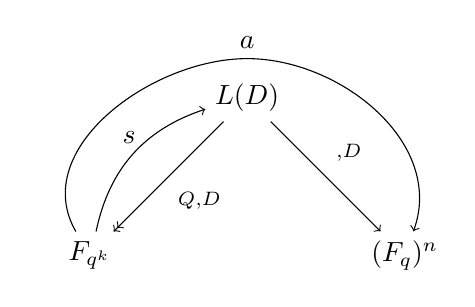
\begin{tikzpicture}
    \node (LD) at (2, 2) {$L(D)$};
    \node (Fqk) at (0, 0) {$\mathbb{F}_{q^k}$};
    \node (Fqn) at (4, 0) {$(\mathbb{F}_{q})^n$};
    \draw[->>] (LD) to (Fqk);
    \draw[->] (LD) to (Fqn);
    \draw[->] (Fqk) to[bend left] (LD);
    \node (s) at (0.5, 1.5) {$s$};
    \node (evQ) at (1.4, .7) {$\ev_{Q, D}$};
    \node (evP) at (3.3, 1.3) {$\ev_{\Pcal, D}$};
    \draw[->] (Fqk) to[out=120,in=180](2, 2.5) to[out=0, in=70] (Fqn);
    \node (a) at (2, 2.7) {$a$};
  \end{tikzpicture}
  \end{center}
Observe that $a$ is linear, so we can write
\[ a(x) = (\varphi_1(x), \dots, \varphi_n(x)) \]
where $\varphi_i:\mathbb{F}_{q^k}\to\mathbb{F}_{q}$ is a linear form, namely $\varphi_i(x)=f_x(P_i)$.

  Similarly, since the map $\ev_{\Pcal, tD}$ is injective, it admits a left inverse, \ie a linear
  map 
  \[
    r: (\mathbb{F}_{q})^n \to L(tD)
  \]
  such that 
  \[r\circ\ev_{\Pcal, tD} = \Id_{L(tD)}.
  \]
We also let $b: (\mathbb{F}_{q})^n \to \mathbb{F}_{q^k}$
  be the composite map $b = \ev_{Q, tD}\circ r$.   The situation is sumed up in the
  following drawing.
  \begin{center}
  \begin{tikzpicture}
    \node (LtD) at (2, 2) {$L(tD)$};
    \node (Fqk) at (0, 0) {$\mathbb{F}_{q^k}$};
    \node (Fqn) at (4, 0) {$(\mathbb{F}_{q})^n$};
    \draw[right hook->] (LtD) to (Fqn);
    \draw[->] (LtD) to (Fqk);
    \draw[->] (Fqn) to[bend right] (LtD);
    \node (evP) at (2.5, .7) {$\ev_{\Pcal, tD}$};
    \node (s) at (3.6, 1.5) {$r$};
    \node (evQ) at (1.2, .4) {$\ev_{Q, tD}$};
    \draw[->] (Fqn) to[out=60,in=0](2, 2.5) to[out=180, in=120] (Fqk);
    \node (d) at (2, 2.7) {$b$};
  \end{tikzpicture}
\end{center}
The map $b$ is linear, so there are $b_1, \dots, b_n$ in
  $\mathbb{F}_{q^k}$ such that, for all $y=(y_1, \dots, y_n)\in(\mathbb{F}_{q})^n$,
  \[
    b(y) = \sum_{i=1}^n y_i b_i.
  \]

Now for $x,\dots,x_t\in\mathbb{F}_{q^k}$, let
  \[
    p = (p_1,\dots,p_n) = ((\prod_{j=1}^tf_{x_j})(P_1), \dots, (\prod_{j=1}^tf_{x_j})(P_n))
  \]
in $(\mathbb{F}_{q})^n$  be the coordinatewise product of the vectors $a(x_1)$, ..., $a(x_t)$.
Then
\[
  h = r(p)
\]
is an element of $L(tD)$ such that $h(P_i) = p_i = (\prod_{j=1}^tf_{x_j})(P_i)$ for all $i$.
Since the map $\ev_{\Pcal, tD}$ is injective, this forces
\[
  h = \prod_{j=1}^tf_{x_j}.
\]
Then, we have
\begin{equation*}
b(p) = \ev_{Q, tD}(r(p))
  = \ev_{Q, tD}(h)
  = h(Q)
  = \prod_{j=1}^t f_{x_j}(Q)
  = \prod_{j=1}^t x_j.
\end{equation*}
But we also have
\[
  b(p) = \sum_{i=1}^np_ib_i=\sum_{i=1}^n(\prod_{j=1}^tf_{x_j}(P_i))b_i=\sum_{i=1}^n(\prod_{j=1}^t\varphi_i(x_j))b_i
\]
and finally we get a symmetric formula for $m_t$:
\[
  \prod_{j=1}^t x_j = \sum_{i=1}^n(\prod_{j=1}^t\varphi_i(x_j))b_i.
\]
\end{proof}
Now that we have a method to find formulas, we have to prove that
Conditions~\ref{cond:1}~and~\ref{cond:2} can be satisfied.
Proposition~\ref{prop:numerical} gives sufficient assumptions to obtain these
conditions.
\begin{prop}
\label{prop:numerical}
Let $F/\mathbb{F}_{q}$ be an algebraic function field of genus $g$.
Assume that $F$ admits a place $Q$ of degree $k$, and a set $\mathcal{S}$ of places of degree $1$ of cardinality
\[
  |\mathcal{S}|\geq (k+g-1)t+1.
\]
Then we have
\[ \musym_q(k,m_t)\leq kt+(g-1)(t-1). \]
\end{prop}
\begin{proof}
Set $n=kt+(g-1)(t-1)$. We will show that there are places $P_1,\dots,P_n$ in $\mathcal{S}$,
and a divisor $D$ on $F$, such that Proposition~\ref{prop:method} applies,
which gives $\musym_q(k,m_t)\leq n$ as desired.

Using e.g. \cite[Lemma~2.1]{Ballet99} we know $F$ admits a non-special divisor $R$ of degree $g-1$.
By the strong approximation theorem \cite[Thm.~1.6.5]{Stichtenoth09}
we can then find a divisor $D$ linearly equivalent to $R+Q$ and of support disjoint from $Q$ and $\mathcal{S}$.

Then $D-Q$ and $D$ are non-special, with $\ell(D-Q)=0$ and $\ell(D)=k$.
We thus find
\[
  \Ker(\ev_{Q, D}:L(D)\to\mathbb{F}_{q^k}) = L(D-Q) = 0,
\]
so $\ev_{Q, D}$ is injective, hence also surjective by equality of dimensions,
\ie the surjectivity condition~\ref{cond:1} in Proposition~\ref{prop:method} is satisfied.

Likewise, $tD$ is non-special, with $\deg(tD)=(k+g-1)t$ and $\ell(tD)=kt+(g-1)(t-1)$.
Then the evaluation map
\[
\begin{array}{cccc}
\ev_{\mathcal{S}, tD}: & L(tD) & \to & (\mathbb{F}_{q})^{|\mathcal{S}|}\\
  & h & \mapsto & (h(P))_{P\in\mathcal{S}}
\end{array}
\]
has kernel $L(tD-\sum_{P\in\mathcal{S}}P)=0$, because $\deg(tD-\sum_{P\in\mathcal{S}}P)=(k+g-1)t-|\mathcal{S}|<0$.
So $\ev_{\mathcal{S}, tD}$ is injective, with image of dimension $\dim\Img(\ev_{\mathcal{S}, tD})=\ell(tD)=n$.
Then we can find a subset $\Pcal=\{P_1,\dots,P_n\}\subset\mathcal{S}$ of cardinality $n$,
such that $\ev_{\Pcal, tD}: L(tD) \to (\mathbb{F}_{q})^n$ is an isomorphism,
and the injectivity condition~\ref{cond:2} in Proposition~\ref{prop:method} is also satisfied.
\end{proof}

\paragraph{Choice of the curves for $q$ a large enough square.}
Now that we have somewhat easier assumptions to fulfill, that are only based on
the existence of a certain number of places, we prove that we can indeed find
algebraic number fields that satisfy these properties. We first prove it in the
special case, where the cardinality $q$ of the base field $\K$ is large enough
square.
\begin{prop}
\label{prop:asymptsquare}
Let $t$ be given, and assume $q$ is a square, $q\geq(t+2)^2$.
Then we have
\[
\Msym_{q,t}\leq(1+\epsilon_t(q))t
\]
with $\epsilon_t(q)=\frac{t-1}{\sqrt{q}-t-1}$.
\end{prop}
\begin{proof}
We know~\cite{STV92} that there exists a family of function fields
$F_i/\mathbb{F}_q$ of genus $g_i\to\infty$ such that
\begin{enumerate}[(i)]
  \item $\frac{g_{i+1}}{g_i}\to1$
  \item $N_i\sim (\sqrt q - 1)g_i$
\end{enumerate}
where $N_i = \Card\left\{ P\in\mathbb{P}_{F_i}\,|\,\deg P = 1 \right\}$
is the number of places of degree $1$ of $F_i$. We can also assume that the sequence
$g_i$ is increasing. 

For any $k$ let $i(k)$ be the smallest index such that
\[ N_{i(k)} \geq (k + g_{i(k)}-1)t +1. \]
Such an $i(k)$ always exists since by (ii) we have $N_i\sim (\sqrt q - 1)g_i$,
with $\sqrt q - 1>t$.

By definition we thus have
\[ N_{i(k)} \geq (k + g_{i(k)}-1)t +1 > (k + g_{i(k)-1}-1)t +1 > N_{i(k)-1}. \]
As $k\to\infty$ we have $i(k)\to\infty$, and by (i) we get 
\[
  g_{i(k)}\sim g_{i(k)-1},
\]
so by (ii) we also get 
\[
  N_{i(k)}\sim N_{i(k)-1}.
\]
This then gives
\[ \begin{split} N_{i(k)} &\sim (k + g_{i(k)}-1)t +1\\ &\sim (k + g_{i(k)})t \end{split} \]
while by (ii),
\[ N_{i(k)} \sim (\sqrt q - 1)g_{i(k)}. \]
From these two relations we deduce
\[ g_{i(k)} \sim \frac{t}{\sqrt{q}-1-t}k. \]
For $k$ large enough this implies in particular $2g_{i(k)} +1 \leq q^{(k-1)/2}(\sqrt q-1)$,
so $F_{i(k)}$ admits a place of degree $k$ by~\cite[Cor.~5.2.10]{Stichtenoth09}.

From this we are allowed to apply Proposition~\ref{prop:numerical} to $F_{i(k)}$, which gives
\[ \musym_q(k,m_t)\;\leq\; kt+(g_{i(k)}-1)(t-1)\;\sim\; kt+g_{i(k)}(t-1)\;\sim\; kt(1+\epsilon_t(q)) \]
as desired.
\end{proof}
\begin{cor}
\label{cor:asymptsquare}
For $q$ a square, $q\geq(t+3)^2$ we have
\[
\Mhyp_{q,t}\leq(1+\epsilon_{t+1}(q))(t+1),
\]
and in particular we have
\[ \Mtri_q\leq 3\left(1+\frac{2}{\sqrt{q}-4}\right) \]
for $q$ a square, $q\geq 25$.
\end{cor}

\paragraph{Conclusion for arbitrary $q$.}
Finally, we complete our objective of proving that the symmetric multilinear
complexity is linear in the degree of the extension by extending the previous
result to arbitrary $q$.

% TODO
% ====
%
% Re-write the first part of this proof. Also what happens with the linear forms
% phi_i in the proof ? They are linear forms over F_{q^{dk}} and not
% F_{q^k}. Could this be a problem?

\begin{lm}
\label{lemma:basechange}
Let $q$ be a prime power. Then for any integers $t,d,k$ we have
\[ \musym_q(k,m_t)\leq\musym_q(dk,m_t)\leq\musym_q(d,m_t)\musym_{q^d}(k,m_t). \]
\end{lm}
\begin{proof}
For the inequality on the left, there is nothing to prove if $\musym_q(dk,m_t)=\infty$.
So let us assume $m_t^{\mathbb{F}_{q^{dk}}/\mathbb{F}_{q}}$ admits a symmetric multiplication formula of length $n=\musym_q(dk,m_t)$, \ie
\[\forall x_1,\dots,x_t\in\mathbb{F}_{q^{dk}},\quad x_1\cdots x_t = \sum_{i=1}^{n}\varphi_i(x_1)\cdots\varphi_i(x_t)a_i \]
for linear forms $\varphi_i:\mathbb{F}_{q^{dk}}\to\mathbb{F}_{q}$ and elements $a_i\in\mathbb{F}_{q^{dk}}$.
Choose a linear projection
\[ p:\mathbb{F}_{q^{dk}}\to\mathbb{F}_{q^{k}} \]
left inverse for the inclusion $\mathbb{F}_{q^{k}}\subseteq\mathbb{F}_{q^{dk}}$.
Then we get
\[\forall x_1,\dots,x_t\in\mathbb{F}_{q^{k}},\quad x_1\cdots x_t = p(x_1,\dots,x_t) = \sum_{i=1}^{n}\varphi_i(x_1)\cdots\varphi_i(x_t)p(a_i) \]
which is a symmetric multiplication formula of length $n$ for $m_t^{\mathbb{F}_{q^{k}}/\mathbb{F}_{q}}$.

Likewise, for the inequality on the right, there is nothing to prove if $\musym_q(d,m_t)=\infty$ or $\musym_{q^d}(k,m_t)=\infty$.
So let us assume $m_t^{\mathbb{F}_{q^{d}}/\mathbb{F}_{q}}$ and $m_t^{\mathbb{F}_{q^{dk}}/\mathbb{F}_{q^{d}}}$ admit symmetric multiplication formulae of length $r=\musym_q(d,m_t)$ and $s=\musym_{q^d}(k,m_t)$ respectively, so
\vspace{-.5\baselineskip}

\[\forall y_1,\dots,y_t\in\mathbb{F}_{q^{d}},\quad y_1\cdots y_t = \sum_{u=1}^{r}\psi_u(y_1)\cdots\psi_u(y_t)b_u \]
\vspace{-1.5\baselineskip}

\[\forall z_1,\dots,z_t\in\mathbb{F}_{q^{dk}},\quad z_1\cdots z_t = \sum_{v=1}^{s}\chi_v(z_1)\cdots\chi_v(z_t)c_v \]
\vspace{-.5\baselineskip}

\noindent for linear forms $\psi_u:\mathbb{F}_{q^{d}}\to\mathbb{F}_{q}$, $\chi_v:\mathbb{F}_{q^{dk}}\to\mathbb{F}_{q^{d}}$ and elements $b_u\in\mathbb{F}_{q^{d}}$, $c_v\in\mathbb{F}_{q^{dk}}$.
Then setting $y_1=\chi_v(z_1)$, ..., $y_t=\chi_v(z_t)$ we find
\[\forall z_1,\dots,z_t\in\mathbb{F}_{q^{dk}},\quad z_1\cdots z_t = \sum_{v=1}^{s}\sum_{u=1}^{r}(\psi_u\circ\chi_v)(z_1)\cdots(\psi_u\circ\chi_v)(z_t)\cdot(b_uc_v) \]
which is a symmetric multiplication formula of length $rs$ for $m_t^{\mathbb{F}_{q^{dk}}/\mathbb{F}_{q}}$.
\end{proof}


\begin{thm}
Let $t\geq2$ be an integer and $q$ a prime power.
If $q<t$, then $\musym_q(k,m_t)=\infty$ for all $k\geq2$.

On the other hand, if $q\geq t$,
then $\musym_q(k,m_t)$ grows at most linearly with $k$, \ie we have
\[
\Msym_{q,t}\leq C_t(q)
\]
for some real constant $C_t(q)<\infty$.
\end{thm}
\begin{proof}
If $q<t$ and $k\geq2$, then $\musym_q(k,m_t)=\infty$ follows from Theorem~\ref{th:criterion}.

On the other hand, for $q\geq t$, we have $\musym_q(d,m_t)<\infty$ for any integer $d$.
Choose $d$ such that $q^d$ is a square, $q^d\geq(t+2)^2$.
Then Proposition~\ref{prop:asymptsquare} shows $\musym_{q^d}(k,m_t)$ grows linearly with $k$.
The Theorem then follows thanks to Lemma~\ref{lemma:basechange}, with $C_t(q)=\musym_q(d,m_t)(1+\epsilon_t(q^d))t$.
\end{proof}
\begin{cor}
For $q\geq t+1$ we have
\[
\Mhyp_{q,t}\leq C_{t+1}(q)
\]
and in particular for $q\geq 3$ we have
\[
\Mtri_q\leq C_{3}(q).
\]
\end{cor}

%
